\section{Frequenzbereich}\label{sec:ag3_2}

In der Elektrotechnik arbeitet man oft an Problemen mit sinus-förmigen Schwingungen. Um die Rechnungen dafür zu vereinfachen bietet es sich an diese Probleme nur im Frequenzbereich zu betrachten. 
Im folgenden wird allerdings zuerst eine Lösung für die skalare lineare gewöhnliche Differentialgleichung im Zeitbereich 

\begin{equation}
	x'(t) = f(t,x) := -kx(t) +r(t)
	\label{DGL}
\end{equation}

mit Startwert $x(t_0) = x_0$ und $k > 0$ ermittelt. Die Anregung ist durch $r(t) = \mathrm{cos}(\omega t)$ als sinus-förmige Schwingung gegeben, wobei $\omega$ die Kreisfrequenz ist.
Aus der vorgegebenen allgemeinen Lösung 

\begin{equation}
	x(t)=\mathrm{e}^{-k(t-t_0)} \left(x_0+\int_{t_0}^{t} \mathrm{e}^{k(s-t_0)}r(s)ds\right)
	\label{Ansatz}
\end{equation} 

betrachtet man vorerst nur das Integral und löst dieses.\\
Für die partielle Integrationsregel 

\begin{equation*}
	\int_{a}^{b}f'(x) \cdot g(x)dx = \left[f(x) \cdot g(x)\right]^{b}_{a} - \int_{a}^{b} f(x) \cdot g'(x)dx
\end{equation*}

setzt man nun $f'(x)=\mathrm{e}^{k(s-t_0)}$ und $g(x)=\mathrm{cos}(\omega s)$. Daraus ergibt sich $f(x)=\frac{1}{k}\mathrm{e}^{k(s-t_0)}$ sowie $g'(x)=-\omega \mathrm{sin}(\omega s)$. Eingesetzt ergibt dies 

\begin{equation*}
	\int_{t_0}^{t} \mathrm{e}^{k(s-t_0)}\mathrm{cos}(\omega s)ds = \left[ \frac{\mathrm{e}^{k(s-t_0)}\mathrm{cos}(\omega s)}{k} \right]^{t}_{s=t_0}-\int_{t_0}^{t}-\frac{\omega \mathrm{sin}(\omega s)\mathrm{e}^{k(s-t_0)}}{k} ds.
\end{equation*}

Unter der Annahme $f'(x)=\frac{\mathrm{e}^{k(s-t_0)}}{k}$, $g(x)=-\omega \mathrm{sin}(\omega s)$ wird erneut partiell integriert, damit folgt $f(x)=\frac{\mathrm{e}^{k(s-t_0)}}{k^2}$ und $g'(x)=-\omega^2 \mathrm{sin}(\omega s)$. Setzt man die Annahmen in die vorherige Gleichung ein, folgt

\begin{equation*}
	\int_{t_0}^{t} \mathrm{e}^{k(s-t_0)}\mathrm{cos}(\omega s)ds = \left[\frac{\mathrm{e}^{k(s-t_0)} \mathrm{cos}(\omega s)}{k}\right]^{t}_{s=t_0}-\left(-\left[\frac{\omega \mathrm{e}^{k(s-t_0)}\mathrm{sin}(\omega s)}{k^2}\right]^{t}_{s=t_0}-\int_{t_0}^{t}-\frac{\omega^2 \mathrm{e}^{k(s-t_0)}\mathrm{cos}(\omega s)}{k^2}ds\right)
\end{equation*} 

dies weiter vereinfacht führt zu 

\begin{equation*}
	\int_{t_0}^{t}\mathrm{e}^{k(s-t_0)}\mathrm{cos}(\omega s)ds = \left[\frac{\mathrm{e}^{k(s-t_0)} \mathrm{cos}(\omega s)}{k}\right]^{t}_{s=t_0} +\left[\frac{\omega\mathrm{e}^{k(s-t_0)} \mathrm{sin}(\omega s)}{k^2}\right]^{t}_{s=t_0}-\frac{\omega^2}{k^2} \int_{s=t_0}^{t}\mathrm{e}^{k(s-t_0)}\mathrm{cos}(\omega s)ds.
\end{equation*}
	
Das Ausgangsintegral findet sich nun sowohl auf der linken, als auch auf der rechten Seite der Gleichung wieder. Die Formel

\begin{equation*}
	\int_{t_0}^{t}\mathrm{e}^{k(s-t_0)}\mathrm{cos}(\omega s)ds \cdot \left(\frac{k^2+\omega^2}{k^2}\right) = \left[\frac{\mathrm{e}^{k(s-t_0)} \mathrm{cos}(\omega s)}{k}\right]^{t}_{s=t_0}+\left[\frac{\omega \mathrm{e}^{k(s-t_0)} \mathrm{sin}(\omega s)}{k^2}\right]^{t}_{s=t_0}
\end{equation*}

ergibt sich durch das Zusammenfassen der beiden gleichen Integrale auf einer Seite. Dividieren durch $\frac{k^2+\omega^2}{k^2}$ und das einsetzen der Integrationsgrenzen führt zu dem Ergebnis des Integrals 

\begin{equation*}
	\int_{t_0}^{t}\mathrm{e}^{k(s-t_0)}\mathrm{cos}(\omega s)ds = 
	\frac{\omega \mathrm{e}^{kt}\mathrm{sin}(\omega t)+k\mathrm{e}^{kt}\mathrm{cos}(\omega t)}{\mathrm{e}^{kt_0}(\omega^2+k^2)}-\frac{\omega \mathrm{sin}(\omega t_0)+k\mathrm{cos}(\omega t_0)}{\omega^2+k^2}.
\end{equation*}

Somit ist die Lösung für (\ref{Ansatz})

\begin{equation*}
	x(t)=\mathrm{e}^{-k(t-t_0)} \left(x_0+\frac{\omega \mathrm{e}^{kt}\mathrm{sin}(\omega t)+k\mathrm{e}^{kt}\mathrm{cos}(\omega t)}{\mathrm{e}^{kt_0}(\omega^2+k^2)}-\frac{\omega \mathrm{sin}(\omega t_0)+k\mathrm{cos}(\omega t_0)}{\omega^2+k^2}\right),
\end{equation*}

durch das Ausmultiplizieren und Aufteilen in den gedämpften Anteil abhängig vom Startwert $x_0$ sowie sinus-förmige Schwingung, erfüllt

\begin{equation}
	x(t) = \mathrm{e}^{-k(t-t_0)}\left(x_0-\frac{\omega \mathrm{sin}(\omega t_0)+k\mathrm{cos}(\omega t_0)}{\omega^2+k^2}\right)+\frac{\omega \mathrm{sin}(\omega t)+k\mathrm{cos}(\omega t)}{\omega^2+k^2}.
	\label{allgemeineLösung}
\end{equation}

die Differentialgleichung (\ref{DGL}) im Zeitbereich.\\

Nach Berechnung der Differentialgleichung im Zeitbereich folgt nun die Betrachtung im Frequenzbereich. Hierbei wird die Lösung als Kosinus unbekannter Amplitude

\begin{equation*}
	x_{freq} (t) = \Re \left\{\underline{x}\mathrm{e}^{j\omega t}\right\}
\end{equation*}

angenommen, mit $\mathrm{cos}(\omega t) = \Re\left\{\mathrm{e}^{j\omega t}\right\}$ wobei $\underline{x}$ der Phasor ist. Die zeitliche Ableitung 

\begin{equation*}
	x'_{freq}(t) = \Re \left\{j\omega \underline{x} \mathrm{e}^{j\omega t}\right\}
\end{equation*}

wird in (\ref{DGL}) eingesetzt, dies liefert

\begin{equation*}
	\Re \left\{j\omega \underline{x} \mathrm{e}^{j\omega t}\right\} = -k\Re\left\{\underline{x}\mathrm{e}^{j\omega t}\right\} + \Re\left\{\mathrm{e}^{j\omega t}\right\}.
\end{equation*}

Umstellen und Zusammenfassen der Terme ergeben die Gleichung

\begin{equation*}
	\Re \left\{(j\omega \underline{x} + k\underline{x} - 1)\mathrm{e}^{j\omega t}\right\} = 0,
\end{equation*}

somit muss $j\omega \underline{x} + k\underline{x} - 1 = 0$ gelten. Nach $\underline{x}$ aufgelöst erhält man 

\begin{equation*}
	\underline{x} = \frac{k-j\omega}{k^2+\omega^2}.
\end{equation*}

Zur Berechnung der Lösung 
\begin{equation}
x_{freq} (t) = \frac{k\mathrm{cos}(\omega t) + \omega\mathrm{sin}(\omega t)}{k^2+ \omega^2}.
\label{lsgfreq}
\end{equation}

im Frequenzbereich (\ref{DGL}) setzt man den berechneten Phasor $\underline{x}$ und die von der Eulerschen in die Polare Darstellung umgerechneten Werte $\mathrm{e}^{j\omega t} = \mathrm{cos}(\omega t) + j\mathrm{sin}(\omega t)$ in $x_{freq}$ ein.



Zwar wird mit dem Ansatz der Lösung im Frequenzbereich das transiente Anfangsverhalten vernachlässigt, jedoch ist die Lösung, verglichen mit dem Ansatz zum Ermitteln des Zeitbereichs, deutlich leichter und weniger zeitaufwändig, da man nur einmal eine sehr einfache Ableitung berechnen muss.\\


Zusätzlich wird eine Reihenschaltung aus einer Spule und einem Widerstand betrachtet ()LR-Schaltung). Diese wird in LT-Spice gebaut und simuliert. Bei der gegebenen Datei  \texttt{Beispielschaltung2.asc} handelt es sich um eine AC-Simulation, aus der das Verhalten der Schaltung in Abhängigkeit von verschiedenen Frequenzen, in diesem Fall von $f=\SI{100}{\hertz}$ bis $f=\SI{1}{\mega\hertz}$, abgelesen werden kann. 

\begin{figure}[h]
	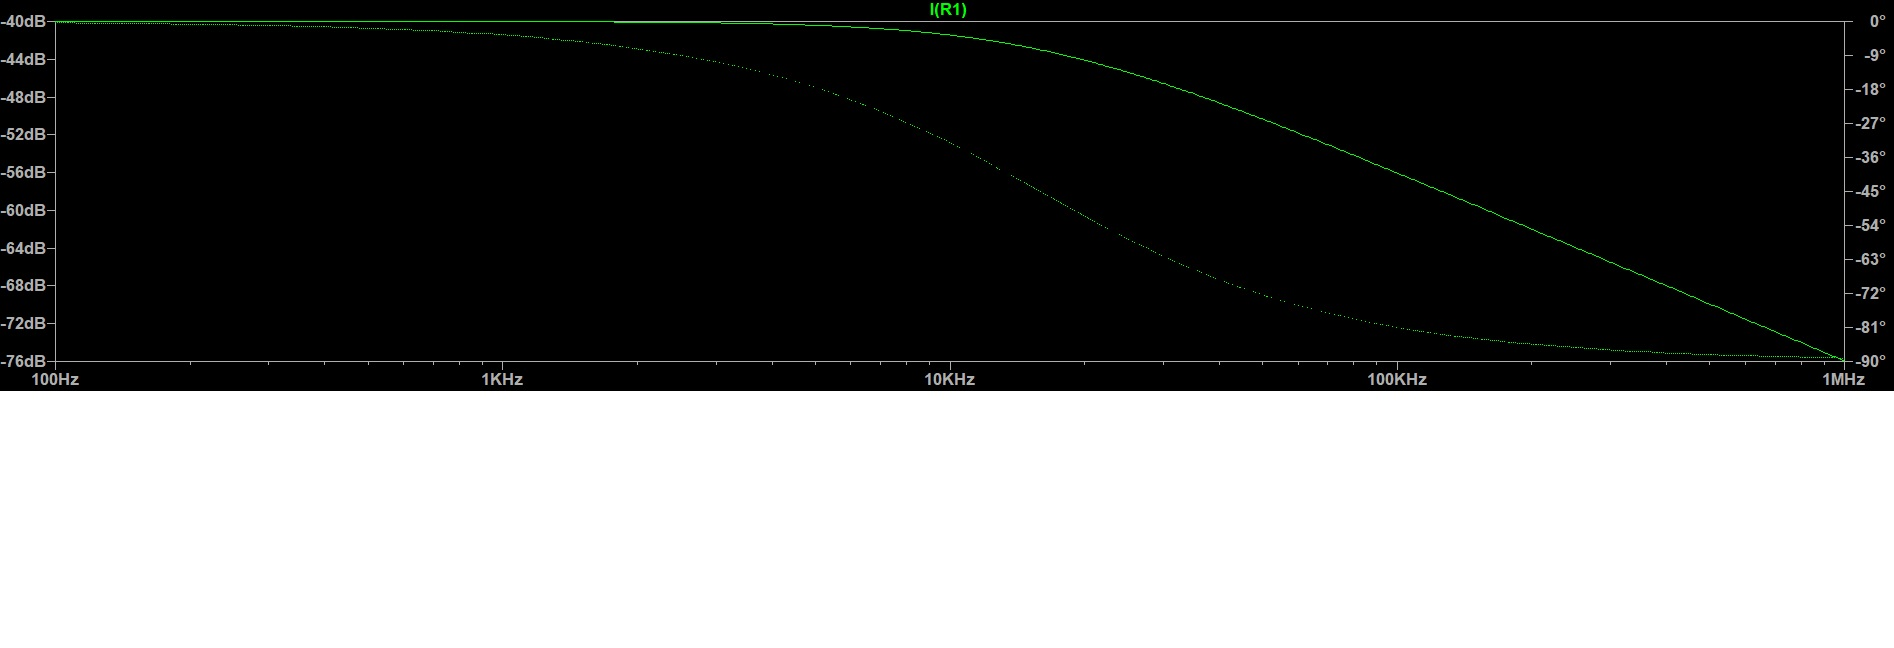
\includegraphics[width=\textwidth]{data/spiceplot32}
	\caption{AC-Simulation aus LT-Spice}
	\label{spiceplot}
\end{figure}

Die Schaltung lässt sich durch die Differentialgleichung

\begin{equation}
	\frac{\mathrm{d}}{\mathrm{d}t}i(t) = -\frac{R}{L}i(t) +\frac{1}{L}u_i(t)
	\label{spezielleDGL}
\end{equation}

beschreiben wobei $R$ der Widerstand, $L$ die Induktivität, $i(t)$ der Strom und $u_i(t)=\mathrm{cos}(\omega t)$ die anregende Spannung ist. Die Lösung für diese Differentialgleichung im Zeitbereich lässt sich mit Hilfe von (\ref{allgemeineLösung}) ermitteln. Hierfür setzt man für $x(t) = i(t)$, $k=\frac{R}{L}$ und für $r(t) = \frac{1}{L}\mathrm{cos}(\omega t)$ ein. Erweitert man im selben Schritt auch noch die Brüche mit $\frac{L}{L}$ so folgt daraus als Lösung für (\ref{spezielleDGL})

\begin{equation*}
	i(t) = \mathrm{e}^{-\frac{R}{L}(t-t_0)}\left(x_0-\frac{L\omega \mathrm{sin}(\omega t_0)+R\mathrm{cos}(\omega t_0)}{L^2\omega^2+k^2}\right)+\frac{L\omega \mathrm{sin}(\omega t)+R\mathrm{cos}(\omega t)}{L^2\omega^2+k^2}.
\end{equation*}

Analog ergibt sich die Lösung im Frequenzbereich durch einsetzen in (\ref{lsgfreq}) mit

\begin{equation*}
	i_{freq} (t) = \frac{R\mathrm{cos}(\omega t) + L\omega\mathrm{sin}(\omega t)}{R^2+ L^2\omega^2}.
\end{equation*}

Die Spannung über dem Widerstand lautet dann nach dem Ohm'schen Gesetz $U=R\cdot I$ und mit der Frequenz $f=\frac{\omega}{2\pi}$

\begin{equation*}
u_{R} (t) = \frac{R\mathrm{cos}(2\pi ft) + 2\pi fL\mathrm{sin}(2\pi ft)}{R^2+ (2\pi fL)^2}R.
\end{equation*}

Das Schaubild für diese Funktion sieht man in Abbildung \ref{spannungplot}.

\begin{figure}[h]
	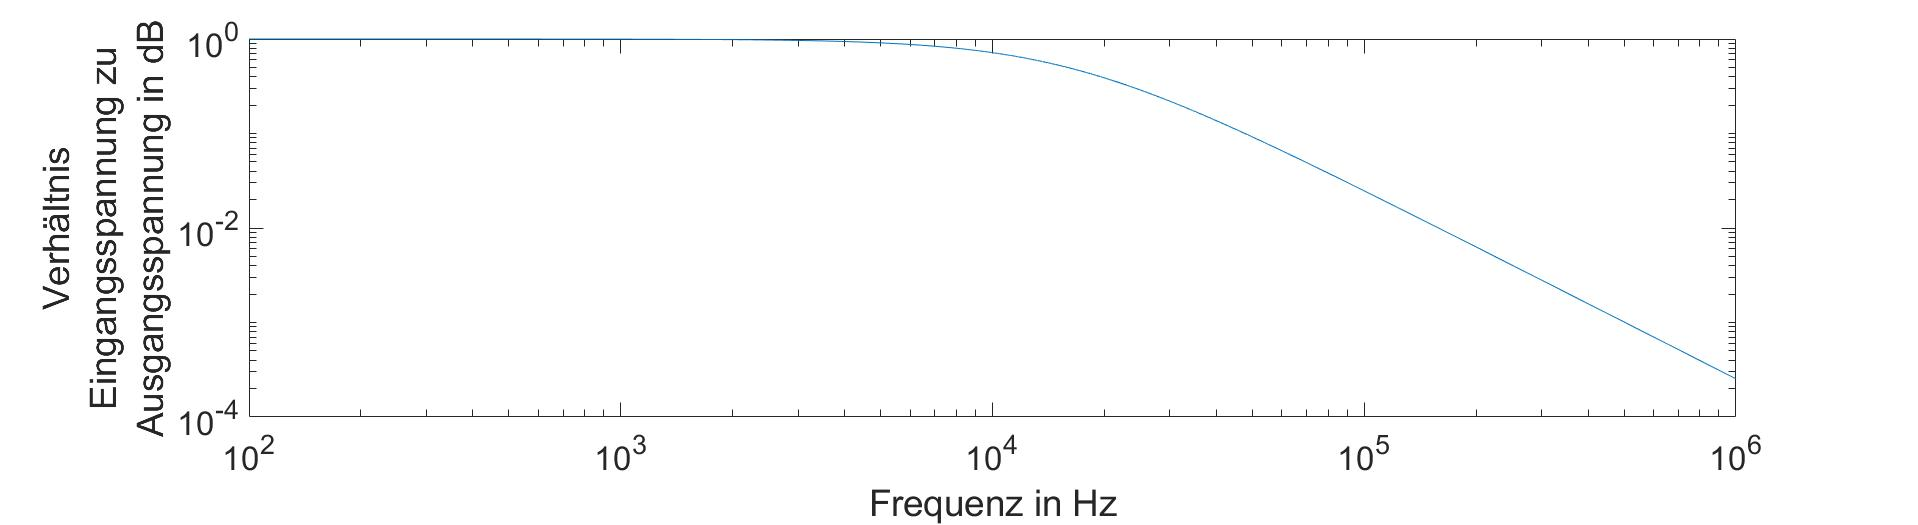
\includegraphics[width=\textwidth]{data/nocheinversuch.jpg}
	\caption{MATLAB-Plot der Spannung über dem Widerstand R}
	\label{spannungplot}
\end{figure}

Anhand des Frequenzgangs fällt auf, dass es sich um eine Schaltung mit Tiefpass-Verhalten handelt, denn bei niedrigen Frequenzen bis ca. $\SI{10}{\kilo\hertz}$ ist die Ausgangsspannung genauso groß wie die Eingangsspannung. Bei hohen Frequenzen nahe $\SI{1}{\mega \hertz}$ ist die Ausgangsspannung deutlich geringer als die Eingangsspannung.




